\documentclass[aspectratio=169]{beamer}
\usepackage{graphicx}
\usepackage{booktabs}
\usepackage{amsmath,amssymb,amsfonts}
\usepackage{multirow}
\usepackage{tikz}
\usepackage{pgfplots}
\usepackage{xcolor}
\usepackage{url}
\usepackage{hyperref}

% Theme settings
\usetheme{Madrid}
\usecolortheme{default}

% PGFPlots compatibility
\pgfplotsset{compat=1.18}

% Custom colors
\definecolor{zjutblue}{RGB}{0,82,155}
\definecolor{zjutred}{RGB}{220,20,60}
\definecolor{zjutgreen}{RGB}{34,139,34}

% Theme colors
\setbeamercolor{structure}{fg=zjutblue}
\setbeamercolor{frametitle}{bg=zjutblue,fg=white}

% Title information
\title[GRCR-Net]{GRCR-Net: A Complex Residual Network with GPR Denoising and Rotational Augmentation for Automatic Modulation Classification}
\subtitle{A Breakthrough Approach for AMC}
\author[Junkai Li]{Junkai Li}
\institute[ZJUT]{College of Information Engineering\\Zhejiang University of Technology}
\date{\today}

% Remove navigation symbols
\setbeamertemplate{navigation symbols}{}

% Page footer settings
\setbeamertemplate{footline}[frame number]

% Begin document
\begin{document}

% The standard and recommended way to generate a title page in Beamer.
% This command uses the information provided above to create the visual title page.
\begin{frame}
    \titlepage
\end{frame}

% Table of contents
\begin{frame}{Outline}
\tableofcontents
\end{frame}

% Section 1: Background and Challenges
\section{Background and Challenges}

\begin{frame}{The Importance of Automatic Modulation Classification}
\begin{columns}
\begin{column}{0.6\textwidth}
\textbf{Critical Applications:}
\begin{itemize}
\item \textbf{Cognitive Radio}: Dynamic spectrum sensing and management
\item \textbf{Spectrum Monitoring}: Radio environment situational awareness
\item \textbf{Military Communications}: Electronic warfare and signal intelligence
\item \textbf{5G/6G Networks}: Intelligent signal processing
\end{itemize}

\vspace{0.5cm}
\textbf{Key Challenge:}
\begin{itemize}
\item Accurate classification under low Signal-to-Noise Ratio (SNR)
\item Preserving I/Q signal phase information
\item Robust performance in complex electromagnetic environments
\end{itemize}
\end{column}
\begin{column}{0.4\textwidth}
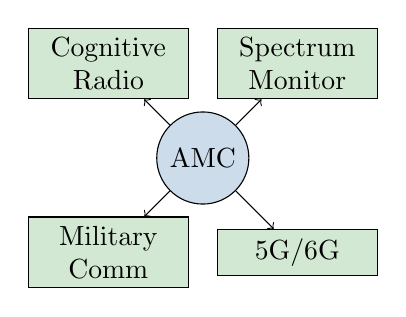
\begin{tikzpicture}[scale=0.8]
\node[draw,circle,fill=zjutblue!20] (amc) at (0,0) {AMC};
\node[draw,rectangle,fill=zjutgreen!20,text width=1.8cm,align=center] (cr) at (-1.5,1.5) {Cognitive\\Radio};
\node[draw,rectangle,fill=zjutgreen!20,text width=1.8cm,align=center] (sm) at (1.5,1.5) {Spectrum\\Monitor};
\node[draw,rectangle,fill=zjutgreen!20,text width=1.8cm,align=center] (mc) at (-1.5,-1.5) {Military\\Comm};
\node[draw,rectangle,fill=zjutgreen!20,text width=1.8cm,align=center] (ic) at (1.5,-1.5) {5G/6G};
\draw[->] (amc) -- (cr);
\draw[->] (amc) -- (sm);
\draw[->] (amc) -- (mc);
\draw[->] (amc) -- (ic);
\end{tikzpicture}
\end{column}
\end{columns}
\end{frame}

\begin{frame}{Core Challenge: Performance Degradation in Low SNR}
\begin{columns}
\begin{column}{0.5\textwidth}
\textbf{Limitations of Existing Methods:}
\begin{itemize}
\item Likelihood-based methods: High computational complexity
\item Feature-based methods: Rely on expert knowledge
\item Deep learning methods: Severe performance drop in low SNR
\end{itemize}

\vspace{0.5cm}
\textbf{Critical Issues:}
\begin{itemize}
\item Noise severely affects signal quality
\item Loss of I/Q signal phase information
\item Data imbalance and poor generalization
\end{itemize}
\end{column}
\begin{column}{0.5\textwidth}
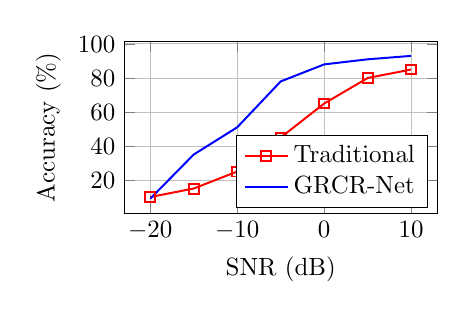
\begin{tikzpicture}[scale=0.9]
\begin{axis}[
    xlabel={SNR (dB)},
    ylabel={Accuracy (\%)},
    grid=major,
    legend pos=south east,
    width=6cm,
    height=4cm
]
\addplot[color=red,mark=square,thick] coordinates {
    (-20,10) (-15,15) (-10,25) (-5,45) (0,65) (5,80) (10,85)
};
\addplot[color=blue,mark=circle,thick] coordinates {
    (-20,9) (-15,35) (-10,51) (-5,78) (0,88) (5,91) (10,93)
};
\legend{Traditional,GRCR-Net}
\end{axis}
\end{tikzpicture}
\end{column}
\end{columns}
\end{frame}

% Section 2: GRCR-Net Innovation Overview
\section{GRCR-Net Innovation Overview}

\begin{frame}{GRCR-Net: Three Core Innovations}
\begin{center}
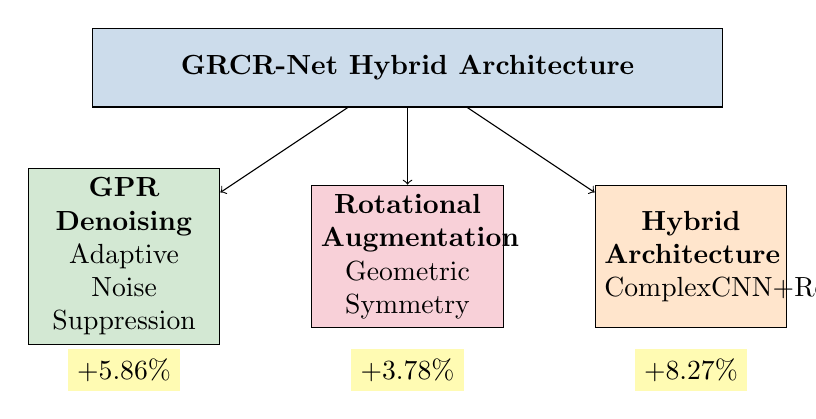
\begin{tikzpicture}[scale=1.2]
% Main framework
\node[draw,rectangle,fill=zjutblue!20,minimum width=8cm,minimum height=1cm] (main) at (0,0) {\textbf{GRCR-Net Hybrid Architecture}};

% Three innovation modules
\node[draw,rectangle,fill=zjutgreen!20,minimum width=2.4cm,minimum height=1.8cm] (gpr) at (-3,-2) {
\begin{minipage}{2.2cm}
\centering
\textbf{GPR Denoising}\\
Adaptive Noise\\Suppression
\end{minipage}
};

\node[draw,rectangle,fill=zjutred!20,minimum width=2.4cm,minimum height=1.8cm] (aug) at (0,-2) {
\begin{minipage}{2.2cm}
\centering
\textbf{Rotational}\\
\textbf{Augmentation}\\
Geometric Symmetry
\end{minipage}
};

\node[draw,rectangle,fill=orange!20,minimum width=2.4cm,minimum height=1.8cm] (hybrid) at (3,-2) {
\begin{minipage}{2.2cm}
\centering
\textbf{Hybrid}\\
\textbf{Architecture}\\
ComplexCNN+ResNet
\end{minipage}
};

% Connection lines
\draw[->] (main) -- (gpr);
\draw[->] (main) -- (aug);
\draw[->] (main) -- (hybrid);

% Performance improvement annotations
\node[fill=yellow!30] at (-3,-3.2) {+5.86\%};
\node[fill=yellow!30] at (0,-3.2) {+3.78\%};
\node[fill=yellow!30] at (3,-3.2) {+8.27\%};
\end{tikzpicture}
\end{center}

\vspace{0.5cm}
\begin{center}
\textcolor{zjutred}{\textbf{Final Performance: 65.38\% Accuracy,\\Surpassing State-of-the-Art}}
\end{center}
\end{frame}

% Section 3: Technical Details
\section{Core Technical Innovations}

\begin{frame}{Innovation 1: Adaptive GPR Denoising Algorithm}
\begin{columns}
\begin{column}{0.6\textwidth}
\textbf{Core Concept:}
\begin{itemize}
\item SNR-adaptive noise estimation
\item Dynamic kernel length-scale adjustment
\item Separate processing of I/Q channels
\end{itemize}

\textbf{Mathematical Foundation:}
\begin{align}
\sigma_n &= \sqrt{\frac{P_r}{2(10^{SNR_{dB}/10}+1)}} \\
L &= \max(L_{min}, L_0(1+SNR/20))
\end{align}

\textbf{Key Advantages:}
\begin{itemize}
\item 7.25\% improvement in low SNR conditions
\item Preserves signal feature integrity
\item High computational efficiency
\end{itemize}
\end{column}
\begin{column}{0.4\textwidth}
\includegraphics[width=\textwidth]{../paper/figure/constellation_denoising.png}
\end{column}
\end{columns}
\end{frame}

\begin{frame}{Innovation 2: Geometric Symmetry-Based Rotational Augmentation}
\begin{columns}
\begin{column}{0.5\textwidth}
\textbf{Theoretical Foundation:}
\begin{itemize}
\item Rotational symmetry of digital modulation constellations
\item Mathematical rigor of complex plane rotation
\item Exploitation of phase invariance
\end{itemize}

\textbf{Implementation:}
\begin{equation}
\begin{bmatrix} s'_I[n] \\ s'_Q[n] \end{bmatrix} = \begin{bmatrix} \cos\theta & -\sin\theta \\ \sin\theta & \cos\theta \end{bmatrix} \begin{bmatrix} s_I[n] \\ s_Q[n] \end{bmatrix}
\end{equation}

\textbf{Augmentation Strategy:}
\begin{itemize}
\item 90°, 180°, 270° rotations
\item 4× training data expansion
\item Applied to symmetric modulation types
\end{itemize}
\end{column}
\begin{column}{0.5\textwidth}
\includegraphics[width=\textwidth]{../paper/figure/constellation.png}
\end{column}
\end{columns}
\end{frame}

\begin{frame}{Innovation 3: Hybrid ComplexCNN-ResNet Architecture}
\begin{center}
\includegraphics[width=0.9\textwidth]{../paper/figure/enhanced_hybrid_model.pdf}
\end{center}

\textbf{Design Principles:}
\begin{itemize}
\item \textbf{Complex Domain Processing}: Direct I/Q signal handling, preserving phase information
\item \textbf{Residual Learning}: Solving gradient vanishing in deep networks
\item \textbf{ModReLU Activation}: Maintaining complex geometric structure
\item \textbf{Lightweight Design}: Balancing performance and computational efficiency
\end{itemize}
\end{frame}

% Section 4: Experimental Results
\section{Experimental Results and Analysis}

\begin{frame}{Dataset and Experimental Setup}
\begin{columns}
\begin{column}{0.6\textwidth}
\textbf{RML2016.10a Dataset:}
\begin{itemize}
\item 11 modulation types
\item SNR range: -20dB to +18dB
\item 128 complex samples per signal
\item Data split: 72\%/8\%/20\%
\end{itemize}

\textbf{Experimental Environment:}
\begin{itemize}
\item Intel Core i9-13900K
\item NVIDIA GeForce RTX 4090 (24GB)
\item TensorFlow 2.17.0 + Keras 3.6.0
\item Ubuntu 24.04.2 LTS
\end{itemize}
\end{column}
\begin{column}{0.4\textwidth}
\begin{table}[h]
\centering
\scriptsize
\begin{tabular}{@{}cc@{}}
\toprule
Modulation & Samples \\
\midrule
8PSK & 22,000 \\
AM-DSB & 22,000 \\
AM-SSB & 22,000 \\
BPSK & 22,000 \\
CPFSK & 22,000 \\
GFSK & 22,000 \\
PAM4 & 22,000 \\
QAM16 & 22,000 \\
QAM64 & 22,000 \\
QPSK & 22,000 \\
WBFM & 22,000 \\
\bottomrule
\end{tabular}
\end{table}
\end{column}
\end{columns}
\end{frame}

\begin{frame}{Baseline Model Performance Comparison}
\begin{columns}
\begin{column}{0.5\textwidth}
\begin{table}[h]
\centering
\begin{tabular}{@{}cc@{}}
\toprule
\textbf{Model Architecture} & \textbf{Accuracy (\%)} \\
\midrule
FCNN & 42.65 \\
CNN2D & 47.31 \\
Transformer & 47.86 \\
CNN1D & 54.94 \\
ResNet & 55.37 \\
ComplexCNN & 57.11 \\
\midrule
\textcolor{zjutred}{\textbf{GRCR-Net}} & \textcolor{zjutred}{\textbf{65.38}} \\
\bottomrule
\end{tabular}
\end{table}
\end{column}
\begin{column}{0.5\textwidth}
\textbf{Key Findings:}
\begin{itemize}
\item ComplexCNN shows natural advantage for I/Q signals
\item ResNet's residual connections improve training stability
\item \textcolor{zjutred}{\textbf{GRCR-Net achieves 8.27\% improvement over best baseline}}
\end{itemize}

\vspace{0.5cm}
\textbf{Performance Breakthrough:}
\begin{itemize}
\item Surpasses existing SOTA methods
\item Consistent improvement across all SNR conditions
\item Exceptional performance in low SNR environments
\end{itemize}
\end{column}
\end{columns}
\end{frame}

\begin{frame}{Ablation Study: Component Contribution Analysis}
\begin{center}
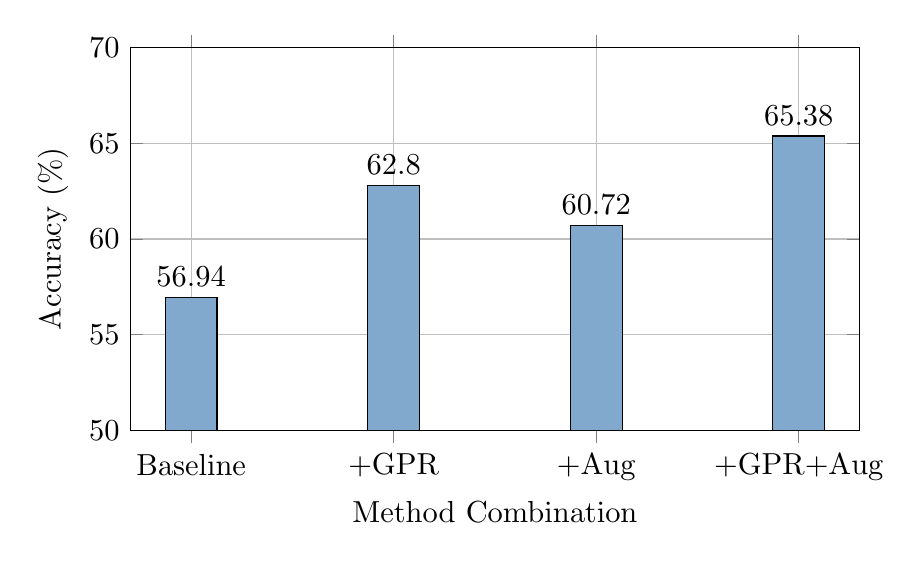
\begin{tikzpicture}[scale=1.1]
\begin{axis}[
    ybar,
    bar width=0.6cm,
    xlabel={Method Combination},
    ylabel={Accuracy (\%)},
    symbolic x coords={Baseline,+GPR,+Aug,+GPR+Aug},
    xtick=data,
    ymin=50,
    ymax=70,
    grid=major,
    width=10cm,
    height=6cm,
    nodes near coords,
    nodes near coords align={vertical},
]
\addplot[fill=zjutblue!50] coordinates {
    (Baseline,56.94)
    (+GPR,62.80)
    (+Aug,60.72)
    (+GPR+Aug,65.38)
};
\end{axis}
\end{tikzpicture}
\end{center}

\textbf{Key Insights:}
\begin{itemize}
\item GPR denoising contributes most: +5.86 percentage points
\item Rotational augmentation provides stable improvement: +3.78 percentage points
\item Synergistic effect of both techniques: total improvement of 8.44 percentage points
\end{itemize}
\end{frame}

\begin{frame}{Performance Across Different SNR Conditions}
\begin{center}
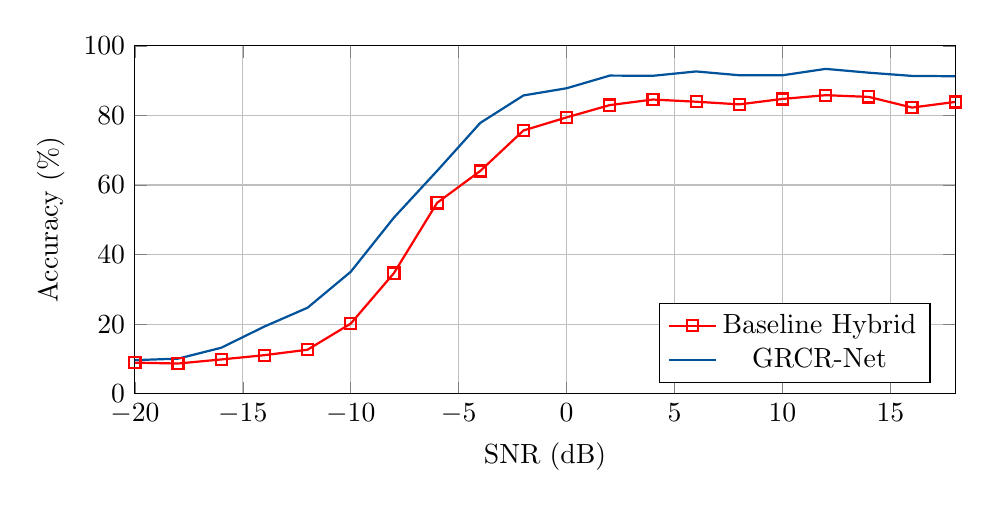
\begin{tikzpicture}[scale=1.0]
\begin{axis}[
    xlabel={SNR (dB)},
    ylabel={Accuracy (\%)},
    grid=major,
    legend pos=south east,
    width=12cm,
    height=6cm,
    xmin=-20,
    xmax=18,
    ymin=0,
    ymax=100
]
\addplot[color=red,mark=square,thick,mark size=2pt] coordinates {
    (-20,8.93) (-18,8.68) (-16,9.85) (-14,11.08) (-12,12.65) (-10,20.15)
    (-8,34.66) (-6,54.86) (-4,64.02) (-2,75.66) (0,79.43) (2,82.96)
    (4,84.56) (6,83.93) (8,83.17) (10,84.73) (12,85.81) (14,85.31)
    (16,82.25) (18,83.87)
};
\addplot[color=zjutblue,mark=circle,thick,mark size=2pt] coordinates {
    (-20,9.65) (-18,10.08) (-16,13.21) (-14,19.31) (-12,24.72) (-10,35.05)
    (-8,50.62) (-6,64.05) (-4,77.84) (-2,85.73) (0,87.80) (2,91.44)
    (4,91.39) (6,92.63) (8,91.54) (10,91.53) (12,93.37) (14,92.27)
    (16,91.35) (18,91.25)
};
\legend{Baseline Hybrid,GRCR-Net}
\end{axis}
\end{tikzpicture}
\end{center}

\textbf{Performance Highlights:}
\begin{itemize}
\item Low SNR (-20dB to -8dB): Average improvement of 7.25 percentage points
\item Medium SNR (-6dB to 4dB): Average improvement of 5.12 percentage points
\item High SNR (6dB to 18dB): Average improvement of 5.07 percentage points
\end{itemize}
\end{frame}

% Section 5: Technical Contributions and Impact
\section{Technical Contributions and Impact}

\begin{frame}{Major Technical Contributions}
\begin{enumerate}
\item \textbf{Adaptive Noise Suppression Technology}
\begin{itemize}
\item First SNR-adaptive GPR denoising algorithm
\item Optimal denoising under different noise conditions
\item Novel approach for complex electromagnetic environments
\end{itemize}

\item \textbf{Geometric Property Data Augmentation Strategy}
\begin{itemize}
\item Exploits inherent symmetry of modulation signals
\item Significantly improves robustness to phase offset
\item Effective solution for data-scarce scenarios
\end{itemize}

\item \textbf{Hybrid Neural Network Architecture Innovation}
\begin{itemize}
\item First fusion of ComplexCNN and ResNet advantages
\item Deep residual learning in complex domain
\item New architectural paradigm for I/Q signal processing
\end{itemize}
\end{enumerate}
\end{frame}

\begin{frame}{Comparison with State-of-the-Art Methods}
\begin{table}[h]
\centering
\scriptsize
\begin{tabular}{@{}lccc@{}}
\toprule
\textbf{Method} & \textbf{Accuracy(\%)} & \textbf{Parameters} & \textbf{Key Technology} \\
\midrule
AMC-Net & 62.51 & Large & Frequency-domain denoising \\
AbFTNet & 64.59 & Large & Multimodal fusion \\
HFECNET-CA & $\sim$60 & Small & Attention mechanism \\
LDCVNN & $\sim$58 & Small & Dual-branch complex network \\
\midrule
\textcolor{zjutred}{\textbf{GRCR-Net}} & \textcolor{zjutred}{\textbf{65.38}} & \textcolor{zjutred}{\textbf{Medium}} & \textcolor{zjutred}{\textbf{GPR+Rotation+Hybrid}} \\
\bottomrule
\end{tabular}
\end{table}

\vspace{0.5cm}
\textbf{Core Advantages:}
\begin{itemize}
\item \textcolor{zjutgreen}{\textbf{Performance Leadership}}: Surpasses best existing method by 0.79\%
\item \textcolor{zjutgreen}{\textbf{Technical Innovation}}: Organic fusion of three core technologies
\item \textcolor{zjutgreen}{\textbf{Practical Robustness}}: Stable performance in complex environments
\item \textcolor{zjutgreen}{\textbf{Scalability}}: Components can be applied independently
\end{itemize}
\end{frame}

\begin{frame}{Practical Application Value and Prospects}
\begin{columns}
\begin{column}{0.6\textwidth}
\textbf{Direct Application Domains:}
\begin{itemize}
\item \textbf{Cognitive Radio}: Intelligent spectrum sensing and management
\item \textbf{Electronic Warfare}: Signal reconnaissance and identification
\item \textbf{Communication Regulation}: Spectrum monitoring and compliance
\item \textbf{5G/6G Networks}: Intelligent signal processing
\end{itemize}

\textbf{Technology Extension Value:}
\begin{itemize}
\item GPR denoising applicable to other signal processing tasks
\item Hybrid architecture extendable to other complex signal analysis
\item Rotational augmentation suitable for geometrically symmetric data
\end{itemize}
\end{column}
\begin{column}{0.4\textwidth}
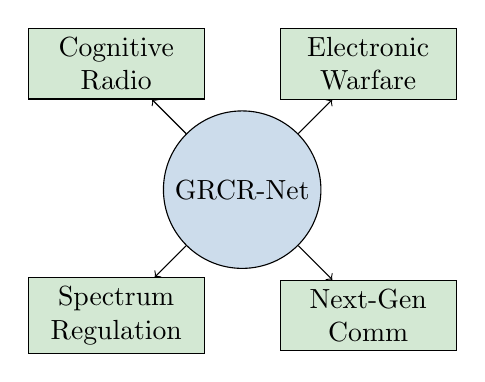
\begin{tikzpicture}[scale=0.8]
% Application scenario diagram
\node[draw,circle,fill=zjutblue!20] (core) at (0,0) {GRCR-Net};
\node[draw,rectangle,fill=zjutgreen!20,text width=2.0cm,align=center] (cr) at (-2,2) {Cognitive\\Radio};
\node[draw,rectangle,fill=zjutgreen!20,text width=2.0cm,align=center] (ew) at (2,2) {Electronic\\Warfare};
\node[draw,rectangle,fill=zjutgreen!20,text width=2.0cm,align=center] (sm) at (-2,-2) {Spectrum\\Regulation};
\node[draw,rectangle,fill=zjutgreen!20,text width=2.0cm,align=center] (ng) at (2,-2) {Next-Gen\\Comm};

\draw[->] (core) -- (cr);
\draw[->] (core) -- (ew);
\draw[->] (core) -- (sm);
\draw[->] (core) -- (ng);
\end{tikzpicture}
\end{column}
\end{columns}
\end{frame}

% Section 6: Conclusion and Future Work
\section{Conclusion and Future Work}

\begin{frame}{Research Summary}
\begin{center}
\textcolor{zjutblue}{\Large \textbf{GRCR-Net: A Breakthrough AMC Method}}
\end{center}

\vspace{0.5cm}
\begin{columns}
\begin{column}{0.5\textwidth}
\textbf{Core Achievements:}
\begin{itemize}
\item[$\checkmark$] Achieved 65.38\% classification accuracy
\item[$\checkmark$] Surpassed existing SOTA methods
\item[$\checkmark$] Exceptional performance in low SNR environments
\item[$\checkmark$] Proposed three core technical innovations
\end{itemize}

\textbf{Technical Breakthroughs:}
\begin{itemize}
\item[$\bullet$] Adaptive GPR denoising algorithm
\item[$\bullet$] Geometric symmetry data augmentation
\item[$\bullet$] Hybrid ComplexCNN-ResNet architecture
\end{itemize}
\end{column}
\begin{column}{0.5\textwidth}
\textbf{Impact Significance:}
\begin{itemize}
\item[$\bullet$] Solution for complex electromagnetic environments
\item[$\bullet$] Advancement of cognitive radio technology
\item[$\bullet$] New insights for signal processing field
\item[$\bullet$] Important theoretical and practical value
\end{itemize}

\textbf{Open Source Contribution:}
\begin{itemize}
\item[$\bullet$] Complete code open-sourced
\item[$\bullet$] Detailed experimental data
\item[$\bullet$] Comprehensive technical documentation
\end{itemize}
\end{column}
\end{columns}
\end{frame}

\begin{frame}{Future Research Directions}
\begin{enumerate}
\item \textbf{Algorithm Optimization and Extension}
\begin{itemize}
\item Explore performance in more complex channel environments
\item Research real-time processing optimization strategies
\item Extend to more modulation types
\end{itemize}

\item \textbf{Technology Fusion and Innovation}
\begin{itemize}
\item Combine with emerging architectures like Transformers
\item Explore multimodal signal fusion
\item Research self-supervised learning methods
\end{itemize}

\item \textbf{Practical Deployment and Applications}
\begin{itemize}
\item Hardware acceleration and edge computing optimization
\item Large-scale real-environment validation
\item Industrial application promotion
\end{itemize}
\end{enumerate}
\end{frame}

\begin{frame}
\centering
\Huge \textcolor{zjutblue}{\textbf{Thank You!}}

\vspace{1cm}
\Large \textcolor{zjutblue}{Questions and Discussion Welcome}

\vspace{1cm}
\normalsize
\textcolor{black}{
Open Source Repository:\\
\url{https://github.com/LJK666666666/radioML-v3}
}
\end{frame}

\end{document}
